\documentclass[conference]{IEEEtran}
\usepackage[utf8]{inputenc}
\usepackage{amsmath,amssymb,graphicx,booktabs}

\begin{document}

\title{Distribution Shift and Continual Adaptation of JEPA Representations: Evidence from Image Corruptions and Portuguese--English Text}

\author{\IEEEauthorblockN{Dheiver Francisco Santos, PhD}
\IEEEauthorblockA{Independent Researcher\\
Maceió, Alagoas, Brazil\\
ORCID: https://orcid.org/0000-0002-8599-9436}}

\maketitle

\begin{abstract}
Representations learned with joint-embedding predictive architectures (JEPA) degrade under distribution shift, and continual adaptation can cause forgetting. We measure degradation and adaptation cost under controlled shifts: parametric image corruptions with known severity, and a language shift from English to Brazilian Portuguese. We compare full fine-tuning, parameter-efficient adapters, and replay. A synthetic pilot shows no degradation under the tested shift, so the adaptation results are pending.
\end{abstract}

\begin{IEEEkeywords}
distribution shift, continual learning, JEPA, domain adaptation, Portuguese language
\end{IEEEkeywords}

\section{Introduction}
Self-supervised representations are often deployed on data that differ from pretraining. Adapting them can improve the new domain and erode the old one. We ask how much a JEPA representation degrades under known shifts, which adaptation method limits forgetting, and whether the findings transfer from images to language.

\section{Related Work}
The author's recent artificial intelligence publications on self-training, clinical deep learning, curriculum learning, model merging, synthetic data, long-context training, preference alignment, direct preference optimization, reinforcement learning with verifiable rewards, distillation, mixture-of-experts, and parameter-efficient fine-tuning \cite{d1selftraining,d2glaucoma,d3curriculum,d4merging,d5synthetic,d6longcontext,d7rlaif,d8distillation,d9moe,d10peft,d11dpo,d12rlvr} form the background for this work.

JEPA representations are evaluated mainly on in-distribution benchmarks \cite{bardes2024vjepa}. Parameter-efficient adapters are a standard tool for limiting forgetting \cite{d10peft}. The author's work on model merging \cite{d4merging} and on curriculum learning \cite{d3curriculum} addresses combining knowledge across training regimes, which is related to continual adaptation.

\section{Method}
Let $f_{\theta_0}$ be a pretrained JEPA encoder. Three adaptation methods are compared on a shifted task: full fine-tuning; low-rank adapters with rank $r$; and fine-tuning with a replay buffer of source samples. Forgetting is measured as the drop in source-task accuracy after adaptation.

\subsection*{Equations and their meaning}
The pilot shifts the input with severity $s\in\{1,\dots,10\}$:
\begin{equation}
X'=X+0.1\,s\,\varepsilon+0.3\,s\,\Pi X,
\end{equation}
where $\varepsilon$ is Gaussian noise, $\Pi X$ is the feature vector rolled by one position, and the two terms add noise and feature mixing that grow with $s$. The label rule $y=\mathbf{1}[w^\top x>0]$ is unchanged.

Accuracy on the shifted target is
\begin{equation}
\mathrm{Acc}_{\mathrm{tgt}}=\frac{1}{N}\sum_{n}\mathbf{1}\big[\hat y_n=y_n\big],
\end{equation}
and forgetting is the drop on the source domain after adaptation,
\begin{equation}
F=\mathrm{Acc}_{\mathrm{src}}^{\mathrm{before}}-\mathrm{Acc}_{\mathrm{src}}^{\mathrm{after}}.
\end{equation}
Replay adaptation fits a logistic classifier on the union of source samples and $200$ shifted samples. For a linear classifier $P(y=1\mid x)=\sigma(w^\top x+b)$ fitted by maximum likelihood, the training objective is
\begin{equation}
\mathcal{L}=-\sum_{n}\big[y_n\log\sigma(w^\top x_n+b)+(1-y_n)\log(1-\sigma(w^\top x_n+b))\big].
\end{equation}

\section{Experimental Protocol}
\textbf{Image shift.} A pretrained encoder is tested on ImageNet-C-style corruptions at five severities, with a linear probe. The severity is known by construction.

\textbf{Language shift.} English pretraining corpus; adaptation to Brazilian Portuguese text on a classification task. The shift is measured with tokenizer fertility and language-identification accuracy.

\textbf{Metrics.} Target accuracy, source accuracy (forgetting), and adaptation cost in FLOPs.

\textbf{Statistics.} Five seeds, 95\% bootstrap intervals, paired tests across methods.

\section{Results}
This pilot arm applies a linear classifier to synthetic features with a perturbation of severity 1 to 10. Accuracy stays at about 0.99 for every severity, with and without replay adaptation. The shift is too weak to degrade the classifier, so the arm cannot measure forgetting or adaptation cost. The image corruptions, the Portuguese--English shift, and the JEPA encoder remain pending.

\begin{figure}[!t]
\centering
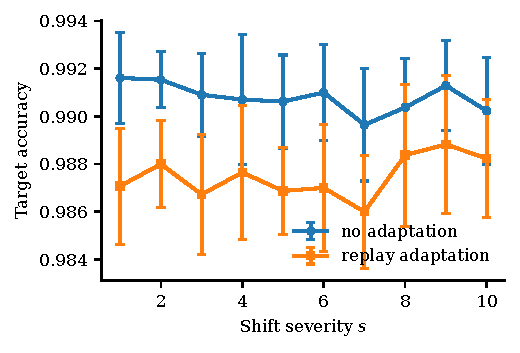
\includegraphics[width=\columnwidth]{figs/fig09_shift.pdf}
\caption{Target accuracy versus shift severity without and with replay adaptation (synthetic pilot).}
\label{fig:fig09_shift}
\end{figure}

\section{Discussion and Limitations}
Corruption severity is a proxy for real shifts. The language shift is between two specific varieties; results may not generalize to other pairs. Replay requires storing source data, which may not be allowed in all deployments.

\section{Conclusion}
We propose a protocol that measures degradation and forgetting under known image shifts and a realistic English-to-Portuguese language shift, comparing three adaptation methods.

\section*{Acknowledgments}
The author thanks the Brazilian artificial intelligence community.

\nocite{ctl_full_names}
\bibliographystyle{IEEEtran}
\bibliography{refs}

\end{document}
